\chapter{Time series metrics and Metric Learning}
\label{sec:Chapter_metrics}
\minitoc

% \noindent Chapeau introductif
%\begin{itemize}
%	\item Rappel : notion de similaire : dans le cadre de la classification, on a un comportement « similaire » pour une même classe. La notion de « similaire » est lié à une notion de distance ou (dis)similarité. 
%	\item Donner les hypothèses de travail : 
%	\begin{itemize}
%		\item Considérons la série temporelle comme étant un objet ordonné.
%		\item les séries temporelles sont de même taille
%		\item les séries temporelles ont la même période d'échantillonnage
%		\item les séries temporelles peuvent être comparés sur l'ensemble des valeurs, sur une partie des valeurs, sur un ensemble de fenêtre (fréquences, etc.)
%	\end{itemize}
%	\item On va définir dans la suite la notion de métrique, d'alignement, de localité pour des séries temporelles.
%	\item Mettre un graphique (dit GRAPHIQUE GENERAL) qui prend 5 séries temporelles que l'on va utiliser pour la suite : proche en valeur, proche en forme, proche en fréquence, proche en valeur avec un délai, proche en forme avec un délai
%\end{itemize}

\fbox{  \parbox{0.9\textwidth}{
		In this chapter, we review different metrics for time series. In classification problems, time series are expected to be similar if they belong to the same class. The concept of similarity among time series is directly linked to the concept of metrics. \\
		
		In the following, we consider time series as an object. They may be compared either on all their observations $x_{it}$, a part of them or in a window. We first recall the properties of a metric. Then, we review three types of metrics (amplitude-based, behavior-based, frequential-based) and kernels adapted to time series. As real time series are subjected to varying delays, we recall the concept of alignment and dynamic programming. We show how these metrics can be used to define either metrics that can capture local characteristics of time series, or metrics that combine multiple modalities. Finally, as $k$-NN performances is directly impacted by the choice of the metric, we review some insights on Metric Learning investigated in the case of static data.
	}  }


%-----------------------------------------------------------------------------
\section{Properties of a metric}
%\begin{itemize}
%	\item Rappeler les propriétés d'une mesure de distance (positivité, symétrique, distinguabilité, inégalité triangulaire)
%	\item Donner les différences entre métriques, distance, dissimilarités, similarités, pseudo-métrique, etc.
%	\item Dans la suite du travail, on va tout assimiler au mot métrique pour une meilleure simplicité
%\end{itemize}

Defining and evaluating adapted metrics for time series has become an active area of research for a wide variety of problems in Machine Learning \cite{Ding2008, Najmeddine2012}. In the following, we suppose that time series have the same lengths $T$ and have been sampled at the same sampling frequency $f_e$. Let $\textbf{x}_i=(x_{i1}, x_{i2}, ..., x_{iT})$ and $\textbf{x}_j=(x_{i1}, x_{i2}, ..., x_{iT})$ be two univariate time series of length $T$. 


A mapping $D:\mathbb{R}^T \times \mathbb{R}^T \rightarrow \mathbb{R}^+$ over a vector space $\mathbb{R}^T$ is called a metric or a distance if for all vectors $\forall \textbf{x}_i, \textbf{x}_j, \textbf{x}_l$, it satisfies the properties:
\begin{enumerate}
	\item {\makebox[6cm]{$D(\textbf{x}_i, \textbf{x}_j) \geq 0$\hfill} (positivity)}
	\item {\makebox[6cm]{$D(\textbf{x}_i, \textbf{x}_j) = D(\textbf{x}_j, \textbf{x}_i)$\hfill} (symmetry)}	
	\item {\makebox[6cm]{$D(\textbf{x}_i, \textbf{x}_j) = 0 \Leftrightarrow  \textbf{x}_i=\textbf{x}_j$\hfill} (distinguishability)}
	\item {\makebox[6cm]{$D(\textbf{x}_i, \textbf{x}_j) D(\textbf{x}_j, \textbf{x}_l) \leq D(\textbf{x}_i, \textbf{x}_l)$\hfill} (triangular inequality)}
\end{enumerate}
A mapping $D$ that satisfies at least properties 1, 2, 3 is called a dissimilarity, and the one that satisfies at least properties 1, 2, 4 a pseudo-metric. Note that for a metric, a dissimilarity and a pseudo metric, if a time series $\textbf{x}_i$ is expected to be closer to $\textbf{x}_j$ than to $\textbf{x}_l$, then $D(\textbf{x}_i,\textbf{x}_j) \leq D(\textbf{x}_i,\textbf{x}_l)$. On the contrary, the mapping $D$ is called a similarity when the time series $\textbf{x}_i$ is expected to be closer to $\textbf{x}_j$ than to $\textbf{x}_l$ and then $D(\textbf{x}_i,\textbf{x}_j) \geq D(\textbf{x}_i,\textbf{x}_l)$. To simplify the discussion in the following, we refer to pseudo-metric and dissimilarity as metrics, pointing out the distinction only when necessary.




%-----------------------------------------------------------------------------
\section{Unimodal metrics for time series}

A large number of distance measures have been proposed in the literature \cite{Montero2014}. Contrary to static data, time series may exibit modalities and specificities due to their temporal nature (e.g., value, shape, frequency, delay, temporal locality). In this section, we review 3 categories of time series metrics used in our work: amplitude-based, frequential-based and behavior-based.



%To illustrate the effect of different metrics, we will consider some toy examples of time series, illustrated in Fig. \ref{fig:ExampleTimeSeriesMetrics}. The objective is to determine which time series is closer to $\textbf{x}_1$. Based on the amplitude of the signals, it is straightforward that $\textbf{x}_2$ is the closest to $\textbf{x}_3$. However, if we consider the shape of the signal, $\textbf{x}_1$ is the closest to $\textbf{x}_3$. $\textbf{x}_1$ and $\textbf{x}_4$ can be considered also as the closest in value if we delete the effect of delays between the two time series. Finally, it seems that $\textbf{x}_1$ and $\textbf{x}_5$ share the same frequential components.
%
%\begin{figure}[h!]
%\centering
%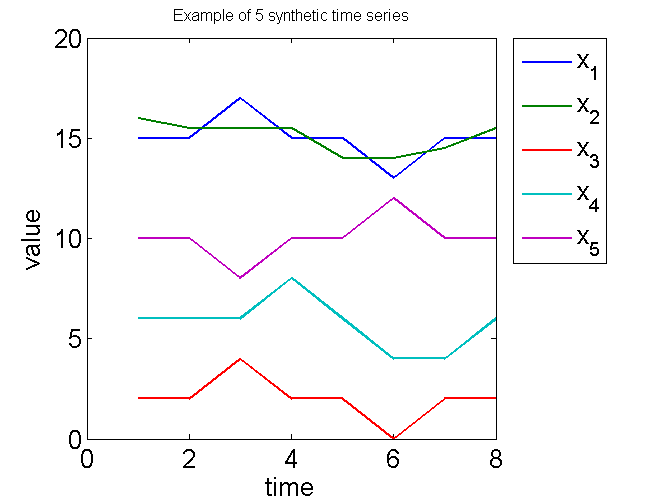
\includegraphics[width=0.6\linewidth]{images/ExampleTimeSeriesMetrics2}
%\caption{An example of 4 time series that can be compared on different distinct modalities. The objective is to determine which time series is closer to $\textbf{x}_3$.}
%\label{fig:ExampleTimeSeriesMetrics}
%\end{figure}
%\todo[  size=\tiny, color=green]{Reparler avec Michèle et Sylvain de la figure. J'aimerai pouvoir trouver 5 séries temporelles qui couvrirait ces cas.}




\subsection{Amplitude-based metrics}
\label{sec:TSmetrics}
%\begin{itemize}
%	\item Distance classiquement utilisée dans la littérature 
%	\item Distance de Minkowski (norm Lp)
%	\item Distance de Mahalanobis (norm pondéré)
%	\item $D_E$	qui est une forme particulière de Minkowski
%	\item Prendre le GRAPHIQUE GENERAL et faire le calcul des distances entre les courbes et montrer que pour 2 courbes qui ont des "amplitudes proches", on obtient une valeur de distance faible. 
%\end{itemize}

The most usual comparison measures are amplitude-based metrics, where time series are compared in the temporal domain on their amplitudes regardless of their behaviors or frequential characteristics. Among these metrics, there are the commonly used Euclidean distance that compares elements observed at the same time \cite{Ding2008}: 
\begin{equation}	
	d_E(\textbf{x}_i,\textbf{x}_j) = \sqrt{\sum\limits_{t=1}^{T} (x_{it}-x_{jt})^2}
\label{eq:A}
\end{equation}
Note that the Euclidean distance is a particular case of the Minkowski $L_p$ norm ($p=2$). An other amplitude-based metric is the Mahalanobis distance \cite{Prekopcsak2012}:
\begin{equation}	
	d_M(\textbf{x}_i,\textbf{x}_j) = (\textbf{x}_i-\textbf{x}_j)'\textbf{M}(\textbf{x}_i-\textbf{x}_j)
	\label{eq:dM}
\end{equation}

\noindent In particular, when $\textbf{M}$ is a diagonal matrix, the previous formula becomes: 
%\textbf{M} &= 	
%\begin{pmatrix}
%	M_1 & 0 & ... & 0 \\
%	0 & M_2 & ... & 0 \\
%	... \\
%	0 & ... & & M_m 
%\end{pmatrix} \\
\begin{align}
M &= 
	\left(
	\begin{array}{ccccc}
	M_1\\
	& ... & & \text{\huge0}\\
	& & M_t & &\\
	& \text{\huge0} & & ... \\
	& & & & M_T
	\end{array}
	\right)	\\
d_M(\textbf{x}_i,\textbf{x}_j) & = \sqrt{\sum\limits_{t=1}^{T} M_t(x_{it}-x_{jt})^2}
\label{eq:dM2}
\end{align}
In practice, the $M_t$ coefficients are often set as the variance of the value on the corresponding dimension. \mycomment[MR]{Plus les données sont imprécises, moins elle est importante}Intuitively, each dimension difference ($x_{it}-x_{jt}$) is weighed by a factor $M_t$. It is also known as the weighted Euclidean distance \cite{McNames2002}. In the following of the work, we consider the standard Euclidean distance $d_E$ as the amplitude-based distance $d_A$.

\begin{figure}[h!]
\centering
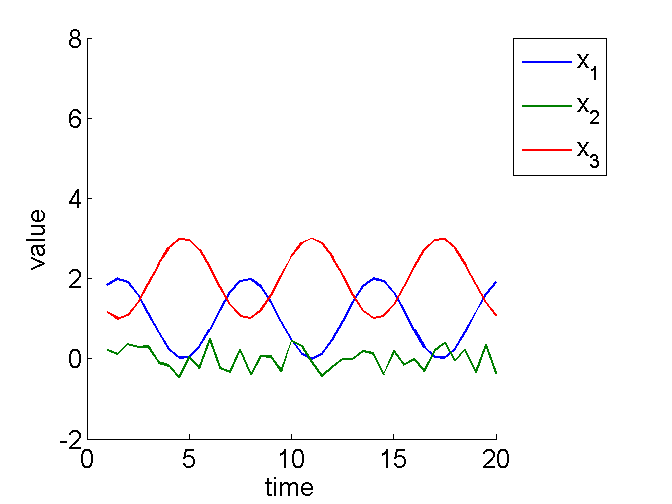
\includegraphics[width=0.7\linewidth]{images/ExampleTimeSeriesMetrics3}
\caption{3 toy time series. Time series in blue and red are two sinusoïdal signals. Time series in green is a random signal.}
\label{fig:ExampleTimeSeriesMetrics3}
\end{figure}

In the example of Fig. \ref{fig:ExampleTimeSeriesMetrics3}, the aim is to determined which time series ($\textbf{x}_2$ or $\textbf{x}_3$) is the closest to $\textbf{x}_1$. The amplitude-based distance $d_A$ states that $\textbf{x}_2$ is closer to $\textbf{x}_1$ than $\textbf{x}_3$ since $d_A(\textbf{x}_1,\textbf{x}_2) = 7.8816 < d_A(\textbf{x}_1,\textbf{x}_3)= 31.2250$.



\subsection{Frequential-based metrics}
%\begin{itemize}
%	\item Dans le cadre du traitement de signal, les gens utilisent des représentations fréquentielles (Fourier, etc.)
%	\item Rappeler la transformée de Fourier (TF) + spectre (module de la TF)
%	\item On peut définir une distance dans la représentation de Fourier.
%	\item Prendre le GRAPHIQUE GENERAL et faire le calcul des distances entre les courbes et montrer que pour 2 courbes qui ont des "spectres proches", on obtient une valeur de distance faible. 
%\end{itemize}
The second category, commonly used in signal processing, relies on comparing time series based on their frequential properties (e.g. Fourier Transform, Wavelet, Mel-Frequency Cepstral Coefficients \cite{Sahidullah2012,Torrence1998,Brigham1967}). In our work, we limit the frequential comparison to Discrete Fourier Transform \cite{Lhermitte2011a}, but other frequential properties can be used as well. Thus, for time series comparison, first the time series $\textbf{x}_i$ are transformed into their Fourier representation $\tilde{\textbf{x}}_i=[\tilde{x}_{i1}, ...,  \tilde{x}_{iF}]$, with $\tilde{x}_{if}$ the complex component at frequential index $f$. The Euclidean distance is then used  between their respective complex number modules $\tilde{x}_{if}$, noted $|\tilde{x}_{if}|$:
\begin{equation}
d_{F}(\textbf{x}_i,\textbf{x}_j) = \sqrt{\sum_{f=1}^{F} 
	(|\tilde{x}_{if}|-|\tilde{x}_{jf}|)^2}
\label{eq:F}
\end{equation}

In the example of Fig. \ref{fig:ExampleTimeSeriesMetrics3}, the frequential-based distance $d_F$ states that the time series $\textbf{x}_3$ is closer to $\textbf{x}_1$ than $\textbf{x}_2$ since $d_F(\textbf{x}_1,\textbf{x}_3) = 0.8519 < d_F(\textbf{x}_1,\textbf{x}_2) = 0.9250$. This can be illustrated in the Frequency domain (Fig. \ref{fig:ExampleTimeSeriesMetrics3_freq})

%\begin{figure}[h!]
%	\centering
%	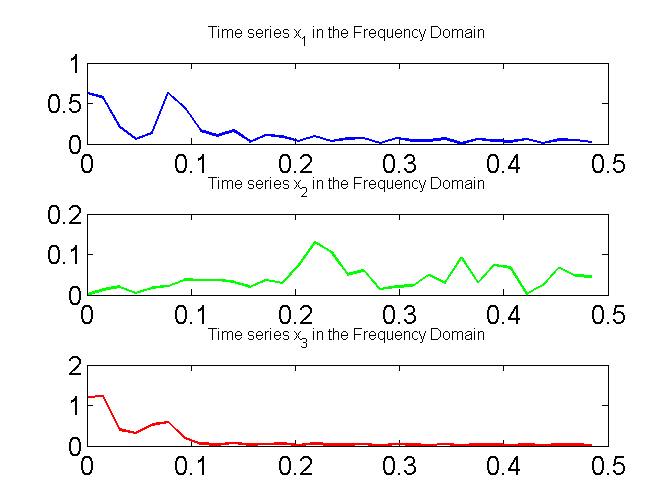
\includegraphics[width=0.7\linewidth]{images/ExampleTimeSeriesMetrics3_freq}
%	\caption{Frequency representation of the signal from Fig. \ref{fig:ExampleTimeSeriesMetrics3}. The spectrum (based on the comparison between frequencies) shows more similarities between signal $\textbf{x}_1$ (blue) and $\textbf{x}_3$ (red) than in the temporal domain (based on the comparison between temporal time t).}
%	\label{fig:ExampleTimeSeriesMetrics3_freq}
%\end{figure}
\missingfigure{Ajouter la représentation fréquentielle des signaux}


\subsection{Behavior-based metrics}
%\begin{itemize}
%	\item Intuition : expliquer ce que signifie "2 séries temporelles sont proches en forme".
%	\item Dans la littérature classique, on trouve la corrélation de Pearson
%	\item Récemment, Douzal \& al. propose une généralisation: cort
%	\item Transformer la cort en mesure de dissimilarité
%	\item Prendre le GRAPHIQUE GENERAL et faire le calcul des distances entre les courbes et montrer que pour 2 courbes qui ont des "formes proches", on obtient une valeur de distance faible. 
%\end{itemize}

The third category of metrics aims to compare time series based on their shape or behavior despite the range of their amplitudes. By time series of similar behavior, it is generally intended that for all temporal window $[t,t']$, they increase or decrease simultaneously with the same growth rate. On the contrary, they are said of opposite behavior if for all $[t,t']$, if one time series increases, the other one decreases and (vise-versa) with the same growth rate in absolute value. Finally, time series are considered of different behaviors if they are not similar, nor opposite. Many applications refer to the Pearson correlation~\cite{Abraham2010a,Benesty2009} for behavior comparison. A generalization of the Pearson correlation is introduced in~\cite{AhlameDouzal-Chouakria2011}: 
\begin{equation}	
	cort_r(\textbf{x}_i,\textbf{x}_j) = 
	\frac{
		\sum 
		{
			(x_{it}-x_{it'})
			(x_{jt}-x_{jt'})
		}
	}
	{
		\sqrt{
			\sum 
			{(x_{it}-x_{it'})^2}
		} 
		\sqrt{
			\sum 
			{(x_{jt}-x_{jt'})^2}
		} 	 
	}
\label{eq:corTr}
\end{equation}

\noindent where $|t-t'| \leq r$, $r \in [1,..., T-1]$. The parameter $r$ can be tuned or fixed a priori. It measures the importance of noise in data. For non-noisy data, low orders $r$ is generally sufficient. For noisy data, the practitioner can either use de-noising data technics (Kalman or Wiener filtering \cite{Kalman1960,WienerN1942}), or fix a high order $r$.

The temporal correlation $cort$ computes the sum of growth rate between $\textbf{x}_i$ and $\textbf{x}_j$ between all pairs of values observed at $[t ,t']$ for $t' \leq t+r$ (r-order differences). The value $cort_r(\textbf{x}_i,\textbf{x}_j) = 1$ means that $\textbf{x}_i$ and $\textbf{x}_j$  have similar behavior. The value $cort_r(\textbf{x}_i,\textbf{x}_j) = -1$ means that $\textbf{x}_i$ and $\textbf{x}_j$ have opposite behavior. Finally, $cort_r(\textbf{x}_i,\textbf{x}_j) = 0$ expresses that their growth rates are stochastically linearly independent (different behaviors). 

When $r=1$, Eq.~\eqref{eq:corTr} leads to the temporal correlation coefficient $cort$ \cite{AhlameDouzal-Chouakria2011}. When $r=T-1$, it leads to the Pearson correlation. As $cort_r$ is a similarity measure, it can be transformed into a dissimilarity measure:
\begin{equation}
	d_B(\textbf{x}_i,\textbf{x}_j) = \frac{1 - cort_r(\textbf{x}_i,\textbf{x}_j)}{2}
	\label{eq:B}
\end{equation}

\begin{figure}[h!]
	\centering
	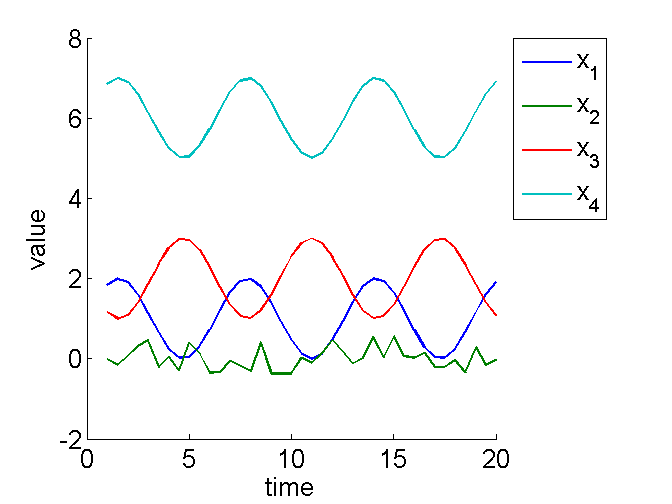
\includegraphics[width=0.7\linewidth]{images/ExampleTimeSeriesMetrics4}
	\caption{The signal from Fig. \ref{fig:ExampleTimeSeriesMetrics3} and a signal $\textbf{x}_4$ which is signal $\textbf{x}_1$ and an added translation. Based on behavior comparison, $\textbf{x}_4$ is the closest to $\textbf{x}_1$.}
	\label{fig:ExampleTimeSeriesMetrics4}
\end{figure}

Now considering Fig. \ref{fig:ExampleTimeSeriesMetrics4}
\begin{align*}
d_B(\textbf{x}_1,\textbf{x}_2) &= 0.477 \\  
d_B(\textbf{x}_1,\textbf{x}_3) &= 1 \\  
d_B(\textbf{x}_1,\textbf{x}_4) &= 0 \\ 
\label{key}
\end{align*}  

\subsection{Other metrics and Kernels for time series}
\todo[inline]{A faire à la fin, pas urgent}
\begin{itemize}
	\item Il existe dans la littérature de nombreuses autres métriques pour les séries temporelles (laisser la porte ouverte).
	\item Certaines métriques sont utilisées dans le domaine temporelle
	\item D'autres métriques sont utilisés dans d'autres représentations (Wavelet, etc.)
	\item Certaines combinent la représentation temporelles et fréquentielles (Représentation spectrogramme en temps-fréquence)
	\item Se baser sur l'article "TSclust : An R Package for Time Series Clustering".
	\item Fermer le cadre : dans la suite de notre travail, on ne va pas les utiliser mais elles pourront être intégrées dans le framework qui suivra au chapitre suivant
\end{itemize}


%-----------------------------------------------------------------------------
\section{Time series alignment and dynamic programming approach}
%\begin{itemize}
%	\item Les données réelles peuvent présenter des délais, des changements de dynamique de l'échelle de temps : extension, compression (dans la limite du raisonnable).
%	\item Il existe des techniques qui permettent de ré-aligner les séries temporelles comme la DTW
%	\item Définir la notion d'alignement
%	\item Présenter la DTW (+ algorithme)
%	\item Présenter les variantes de la DTW
%	\item Dans la suite du travail, on suppose que les séries temporelles sont ré-alignées.
%	\item Prendre le GRAPHIQUE GENERAL et faire le calcul des distances entre les courbes et montrer que pour 2 courbes qui ont des "valeurs proches" mais décalés, on obtient une valeur de distance faible. (prendre DTW standard avec une fonction de coût $D_E$ par exemple)
%\end{itemize}

In some applications, time series needs to be compared at different time $t$ (i.e. energy data \cite{Najmeddine2012}) whereas in others, comparing time series on the same time $t$ is essential (i.e. gene expression \cite{Chouakria2007}). When time series are asynchronous (i.e. varying delays or dynamic changes), they must be aligned before any analysis process. The asynchronous effects can be of various natures: time shifting (phase shift in signal processing), time compression or time dilatation. For example, in the case of voice recognition (Fig. \ref{fig:Voice_Example}), it is straightforward that a same sentence said by two different speakers will produce different time series: one speaker may speak faster than the other; one speaker may take more time on some vowels, etc.

\begin{figure}[h!]
\centering
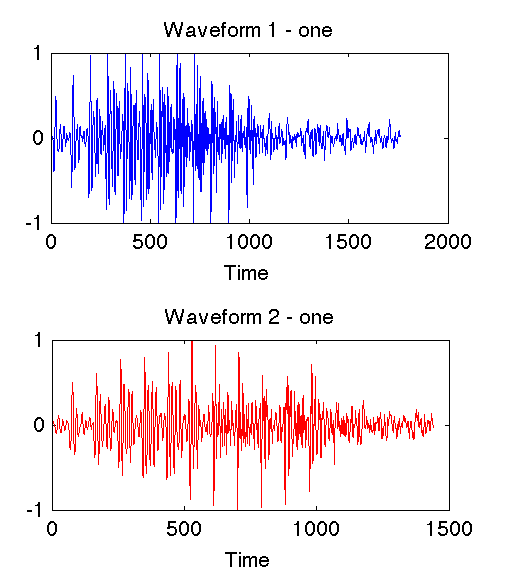
\includegraphics[width=0.5\linewidth]{images/Voice_Example}
\caption{Example of a same sentence said by two different speakers. Time series are shifted, compressed and dilatated in the time.}
\label{fig:Voice_Example}
\end{figure}
\mycomment[MR]{Modifier figure. enlever 'one' et mettre la même échelle temporelle}
To cope with delays and dynamic changes, dynamic programming approach has been introduced \cite{Berndt1994a}. An alignment $\boldsymbol{\pi}$ of length $|\boldsymbol{\pi}|=m$ between two time series $\textbf{x}_i$ and $\textbf{x}_j$ of length $T$ is defined as the set of $m$ ($T \leq m \leq 2T-1$) couples of aligned elements of $\textbf{x}_i$ to $m$ elements of $\textbf{x}_j$:
\begin{equation}
\boldsymbol{\pi} = 
\left(  
(\pi_i(1),\pi_j(1)), 
(\pi_i(2),\pi_j(2)), 
\ldots,
(\pi_i(m),\pi_j(m))
\right) 
\end{equation}
\noindent where the applications $\pi_i$ and $\pi_j$ defined from $\{1, ..., m\}$ to $\{1, ..., T\}$ obey the following boundary monotonicity conditions: 
\begin{align}
& 1 = \pi_i(1) \leq \pi_i(2) \leq ... \leq \pi_i(m) = T \\
& 1 = \pi_j(1) \leq \pi_j(2) \leq ... \leq \pi_j(m) = T 
\end{align}
$\forall l \in \{1, ..., m\}$, 
\begin{align}
& \pi_i(l+1) \leq \pi_i(l)+1 \\
\text{  and  \qquad} & \pi_j(l+1) \leq \pi_j(l)+1 \\
\text{  and  \qquad} & ( \pi_i(l+1)-\pi_i(l) ) - ( \pi_j(l+1)-\pi_j(l)) \geq 1 . 
\end{align}
Intuitively, an alignment $\boldsymbol{\pi}$ defines a way to associate elements of two time series. Alignments can be described by paths in the $T \times T$ grid that crosses the elements of $\textbf{x}_i$ and $\textbf{x}_j$ (Fig. \ref{fig:DTWgrid}). We denote $\boldsymbol{\pi}$ a valid alignment and $A$, the set of all possible alignments between $\textbf{x}_i$ and $\textbf{x}_j$ ($\boldsymbol{\pi} \in A$). To find the best alignment $\boldsymbol{\pi}^*$ between two time series $\textbf{x}_i$ and $\textbf{x}_j$, the Dynamic Time Warping (\textsc{dtw}) algorithm has been proposed \cite{Keogh2004,Salvador}.

\textsc{dtw} requires to choose a cost function $\varphi$ to be optimised, such as a dissimilarity function ($d_A, d_B$, $d_F$, etc.). Classical \textsc{dtw} uses the Euclidean distance $d_A$ (Eq. \ref{eq:A}) as the cost function~\cite{Berndt1994a}. The warp path $\boldsymbol{\pi}$ is optimized for the chosen cost function $\varphi$:
\begin{equation}
\boldsymbol{\pi}^* = \argmin_{\boldsymbol{\pi} \in A} \frac{1}{|\boldsymbol{\pi}|}
\sum_{(t,t') \in \boldsymbol{\pi}} \varphi(x_{it}, x_{jt'})
\label{eq:DTW}
\end{equation}

\noindent When the cost function $\varphi$ is a similarity measure, the optimization involves maximization instead of minimization. When other constraints are applied on $\boldsymbol{\pi}$, Eq. \eqref{eq:DTW} leads to other variants of \textsc{dtw} (Sakoe-Shiba \cite{Sakoe1978a}, Itakura parallelogram \cite{Rabiner1993}). Finally, the warped signals $\textbf{x}_{i,\boldsymbol{\pi}}$ and $\textbf{x}_{j,\boldsymbol{\pi}}$ are defined as:
\begin{align}
\textbf{x}_{i,\boldsymbol{\pi}} 
&= (x_{i\pi_i(1)}, ..., 
x_{i\pi_i(m)}) 			\\	
\textbf{x}_{j,\boldsymbol{\pi}} 
&= (x_{j\pi_j(1)}, ..., 
x_{j\pi_j(m)}) 	
\end{align}

\begin{figure}[h!]
	\centering
	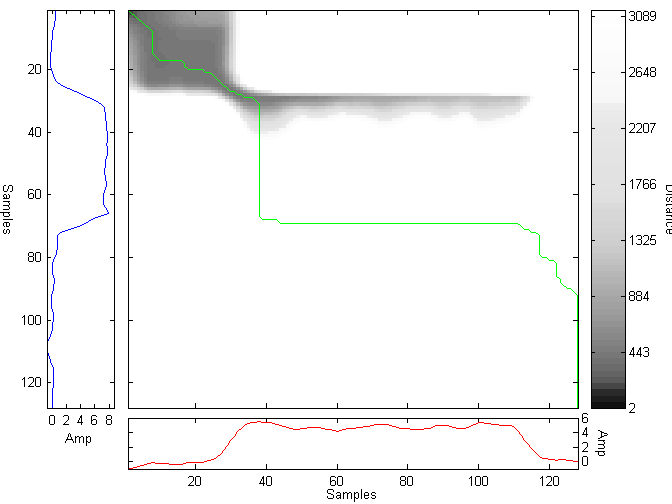
\includegraphics[width=0.5\linewidth]{images/DTWgrid2}
	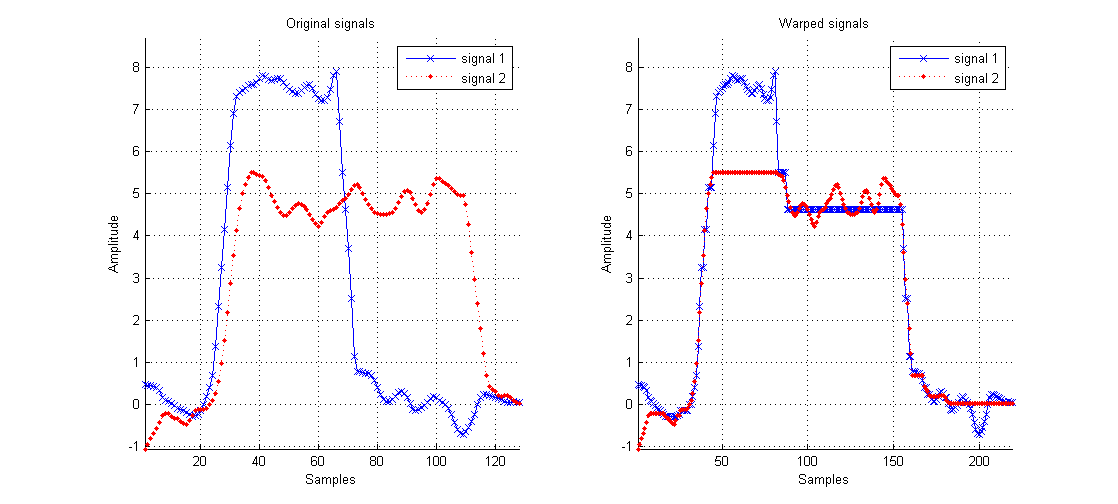
\includegraphics[width=0.9\linewidth]{images/DTWwarpedSignals}
	\caption{Example of {\sc dtw} grid between 2 time series $\textbf{x}_{i}$ and $\textbf{x}_{j}$ (top) and the signals before and after warping (bottom). On the {\sc dtw} grid, the two signals can be represented on the left and bottom of the grid. The optimal path $\boldsymbol{\pi}^*$ is represented in green line and show to associate elements of $\textbf{x}_{i}$ to element of $\textbf{x}_{j}$. Background show in grey scale the value of the considered metric (amplitude-based distance $d_A$ in classical {\sc dtw})}
	\label{fig:DTWgrid}
\end{figure}


The previous metric (amplitude-based $d_A$, behavior-based $d_B$) can be then computed on the warped signals $\textbf{x}_{i,\boldsymbol{\pi}^*}$ and $\textbf{x}_{j,\boldsymbol{\pi}^*}$. In the following, we suppose that the best alignment $\boldsymbol{\pi}^*$ is found. For simplification purpose, we refer $\textbf{x}_{i,\boldsymbol{\pi}^*}$ and $\textbf{x}_{j,\boldsymbol{\pi}^*}$ as $\textbf{x}_{i}$ and $\textbf{x}_{j}$. 


%-----------------------------------------------------------------------------
\section{Multi-scale comparison}
%\begin{itemize}
%	\item Dans le cadre de la classification, on peut avoir des données où l'information qui permet de discriminer une classe d'une autre n'est pas globale mais est localisé sur une partie du signal
%	\item Limite des métriques basiques présentées précédemment (valeur, forme, fréquence) considère la comparaison sur l'intégralité du signal
%	\item On propose la définition de métriques locales. Pour cela, on va découper notre signal. Il existe plusieurs manières de réaliser ce découpage. On va utiliser la dichotomie proposée par Douzal \& al.
%\end{itemize}

In some applications, time series may exhibit similarities among the classes based on local patterns in the signal. Fig. \ref{fig:UMD} illustrates a toy example (UMD dataset) in which the time series of different classes seems to be similar on a global scale. However, at a more locally scale, a characteristic bell (up or down) at the beginning or at the end of the time series allows to differentiate the classes. Also, in massive time series datasets, computing the metric on all time series elements $x_{it}$ might become time consuming. Computing the metric on a smaller part of the signal and not all the time series elements makes the metric computation faster.

\begin{figure}[h!]
	\centering
	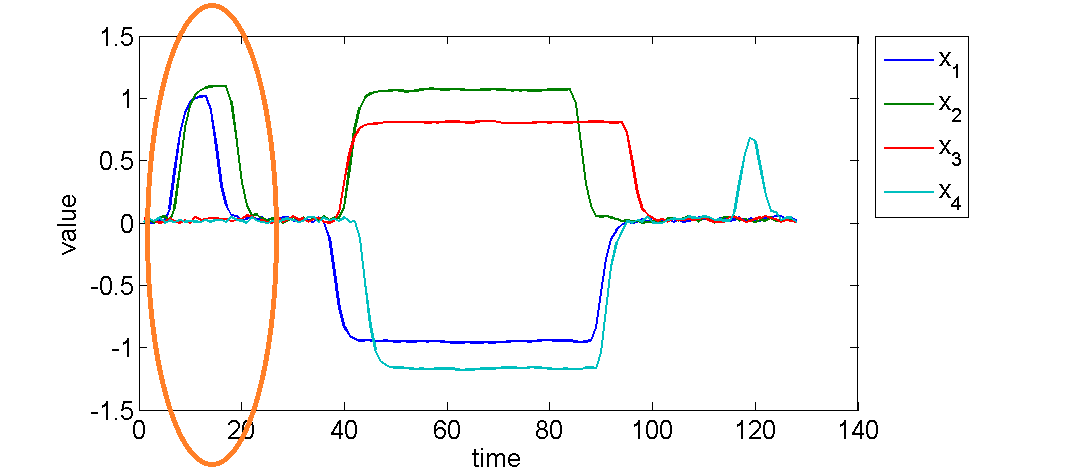
\includegraphics[width=0.8\linewidth]{images/BME_local}
	\caption{Example of 4 time series from the BME dataset, made of 3 classes : Begin, Middle and End. The 'Up' class has a characteristic bell at the beginning of the time series. The 'End' class has a characteristic bell at the end of the time series. The 'Middle' class has no characteristic bell. Orange circle show the region of interest of these bells for the class 'Begin'. This region is local and standard global metric fails to show these characteristics.}
	\label{fig:UMD}
\end{figure}

Localizing patterns of interest in huge time series datasets has become an active area of search in many applications including diagnosis and monitoring of complex systems, biomedical data analysis, and data analysis in scientific and business time series \todo{ref}. A large number of methods have been proposed covering the extraction of local features from temporal windows \cite{Berndt1994a} or the matching of queries according to a reference sequence \cite{Faloutsos1994}. Our work will focus on the computation of local metrics.

It can be noted that the distance measures ($d_A$\footnote{We recall that $d_A$ is the Euclidean distance $d_E$ in our work.}, $d_F$, $d_B$) in Eqs. \ref{eq:A}, \ref{eq:F} and \ref{eq:B} implies systematically the total time series elements $x_{it}$ and thus, restricts the distance measures to capture local temporal differences. In our work, we provide a multi-scale framework for time series comparison. Many methods exist in the literature such as the sliding window or the dichotomy \todo{ref}. We detailed here the latter one.


A multi-scale description is obtained by repeatedly segmenting a time series expressed at a given temporal scale to induce its description at a more locally level. Many approaches have been proposed assuming fixed either the number of the segments or their lengths. In our work, we fix the number of segments and consider a binary segmentation. Let $I=[a;b]$ be a temporal interval of size $(b-a)$. For a strict division (no overlapping), the dichotomy process divide $I$  into two equal intervals at $\frac{b-a}{2}$: the left one $I_L$ and the right $I_R$ one. We add a parameter $\alpha$ that allows to overlap the two intervals $I_L$ and $I_R$, covering discriminating subsequences in the central region of I (around $\frac{b-a}{2}$) and thus avoiding 'border effects':
\begin{align}
	I &= [a;b] \\
	I_L &= [a;a+\alpha(b-a)] \\
	I_R &= [a-\alpha(b-a);b] 
\label{key}
\end{align}
\noindent For $\alpha = 0.6$, the overlap covers $10\%$ of the size of the interval $I$. A multi-scale description is then obtained on computing the usual time series metrics ($d_A$, $d_B$, $d_F$) on the resulting segments $I$, $I_L$ and $I_R$ and by repeating the process on $I_L$ and $I_R$. For a multi-scale amplitude-based comparison based on binary segmentation, Figure \ref{fig:Intervalles} shows the set of involved amplitude-based measures $d^{Is}_A$:
\begin{equation}	
d^{Is}_A(\textbf{x}_i,\textbf{x}_j) = \sqrt{\sum\limits_{t \in Is} (x_{it}-x_{jt})^2}
\label{eq:A2}
\end{equation}
The local behaviors- and frequential- based measures $d^{Is}_B$ and $d^{Is}_F$ are obtained similarly.

\begin{figure}[h!]
\centering
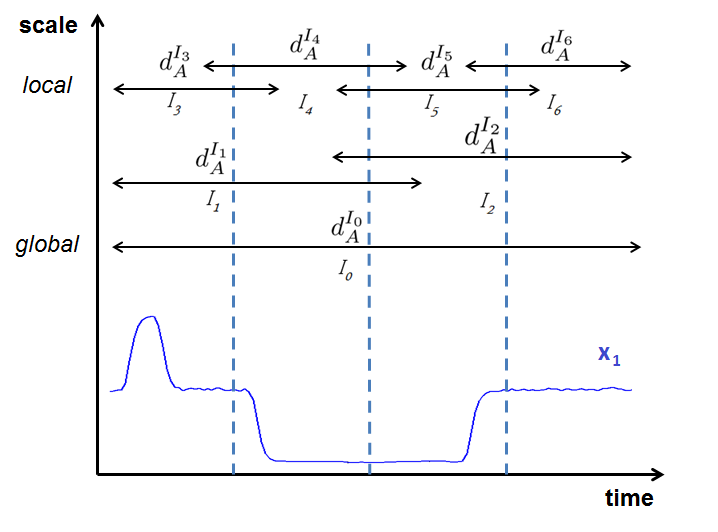
\includegraphics[width=0.8\linewidth]{images/Intervalles2}
\caption{Multi-scale amplitude-based measures $d^{Is}_A$}
\label{fig:Intervalles}
\end{figure}


%\noindent Chapeau introductif
%\begin{itemize}
%	\item Objectif : Trouver une distance, combinaison des distances basiques qui donne une bonne classification $k$-NN sur une base de données.
%	\item Pourquoi une distance combinée? Dans le cadre de données réelles, plusieurs modalités peuvent être impliquées (forme, valeur, fréquence), de manière globale ou locale.
%	\item Dans le cadre des données réelles, plusieurs composantes/modalités peuvent être impliqués (forme, valeur, fréquence). = attribut (feature) en traitement du signal. Hypothèse : valeur sur une série complète, sur un intervalle ou sur une fenêtre (dans le cadre des métriques à base fréquentielle).
%\end{itemize}

%-----------------------------------------------------------------------------
\section{Combined metrics for time series}
%\begin{itemize}
%	\item Certains travaux dans la littérature propose des combinaisons : linéaire, exponentielle, sigmoïde.
%	\item Limites:
%	\begin{itemize}
%		\item Implique que 2 modalités et au niveau global. Pour intégrer d'autres modalités et à d'autres échelles, il faut changer la formule et ajouter de nouveaux hyper-paramètres à optimiser $\rightarrow$ l'apprentissage de ces paramètres est plus long.
%		\item La combinaison est définie a priori
%		\item La combinaison est indépendante de la tâche d'analyse.
%		\item Pour répondre à ces problèmes, certains auteurs proposent d'apprendre une métrique en vue de la tâche d'analyse considérée (classification, régression, clustering).
%	\end{itemize}
%\end{itemize}

In most classification problems, it is not known a priori if time series of a same class exhibits same characteristics based on their amplitude,  behavior or frequential components alone. In some cases, several components (amplitude, behavior and/or frequential) may be implied. 

A first technic considers a classifier for each $p$ metric and combines the decision of the $p$ resulting classifiers. This methods is referred as post-fusion \todo{ref}, not considered in our work. Other propositions show the benefit of involving both behavior and amplitude components through a combination function. They combines the unimodal metrics together to obtain a single metric used after that in a classifier. This is called pre-fusion. The most classical combination functions combines the unimodal metrics (mainly $d_A$ and $d_B$) through linear and geometric functions:
\begin{align}
D_{Lin}(\textbf{x}_i,\textbf{x}_j) &= \alpha d_{B}(\textbf{x}_i,\textbf{x}_j) + (1-\alpha) d_A(\textbf{x}_i,\textbf{x}_j)  \label{eq:DLin}   \\
D_{Geom}(\textbf{x}_i,\textbf{x}_j) &= (d_{B}(\textbf{x}_i,\textbf{x}_j))^\alpha  (d_A(\textbf{x}_i,\textbf{x}_j))^{1-\alpha} \label{eq:DGeom}
\end{align}

\noindent where $\alpha \in [0;1]$ defines the trade-off between the amplitude $d_A$ and the behavior $d_B$ components, and is thus application dependent. In general, it is learned through a grid search procedure. Without being restrictive, these combinations can be extended to take into account more unimodal metrics. \\
More specific work on $d_A$ and $cort$ propose to combine the two unimodal metrics through a sigmoid combination function \cite{AhlameDouzal-Chouakria2011}:
\begin{equation}	
D_{Sig}(\textbf{x}_i,\textbf{x}_j) = \frac{2d_A(\textbf{x}_i,\textbf{x}_j)}{1+\exp(\alpha cort_r(\textbf{x}_i,\textbf{x}_j))}
\label{eq:DSig}
\end{equation}
\noindent where $\alpha$ is a parameter that defines the compromise between behavior and amplitude components. When $\alpha$ is fixed to 0, the metric only includes the value proximity component. For $\alpha \geq 6$, the metric completely includes the behavior proximity component. 

Fig.\ref{fig:ContourLine} illustrates the value of the resulting combined metrics ($D_{Lin}$, $D_{Geom}$ and $D_{Sig}$) in 2-dimensional space using contour plots for different values of the trade-off $\alpha$. For small value of $\alpha$ (=0), the three metrics only includes $d_A$. For high value of $\alpha$ (=1), $D_{Lin}$ and $D_{Geom}$ only includes $d_B$. For $\alpha=6$, $D_{Sig}$ doesn't include completely $cort$. Note that these combinations are fixed and defined independently from the analysis task at hand. Moreover, in the case of $D_{Sig}$, only two variables are taking into account in these combined metrics and the component $cort_r$ can be seen as a penalizing factor of $d_A$. It doesn't represent a real compromise between value and behavior components. Finally, by adding metrics, the grid search to find the best parameters can become time consuming.
% To overcome these limits, other authors propose to learn the metric $D$ for a robust $k$-NN classifier. 

\begin{figure}[h!]
	\centering
	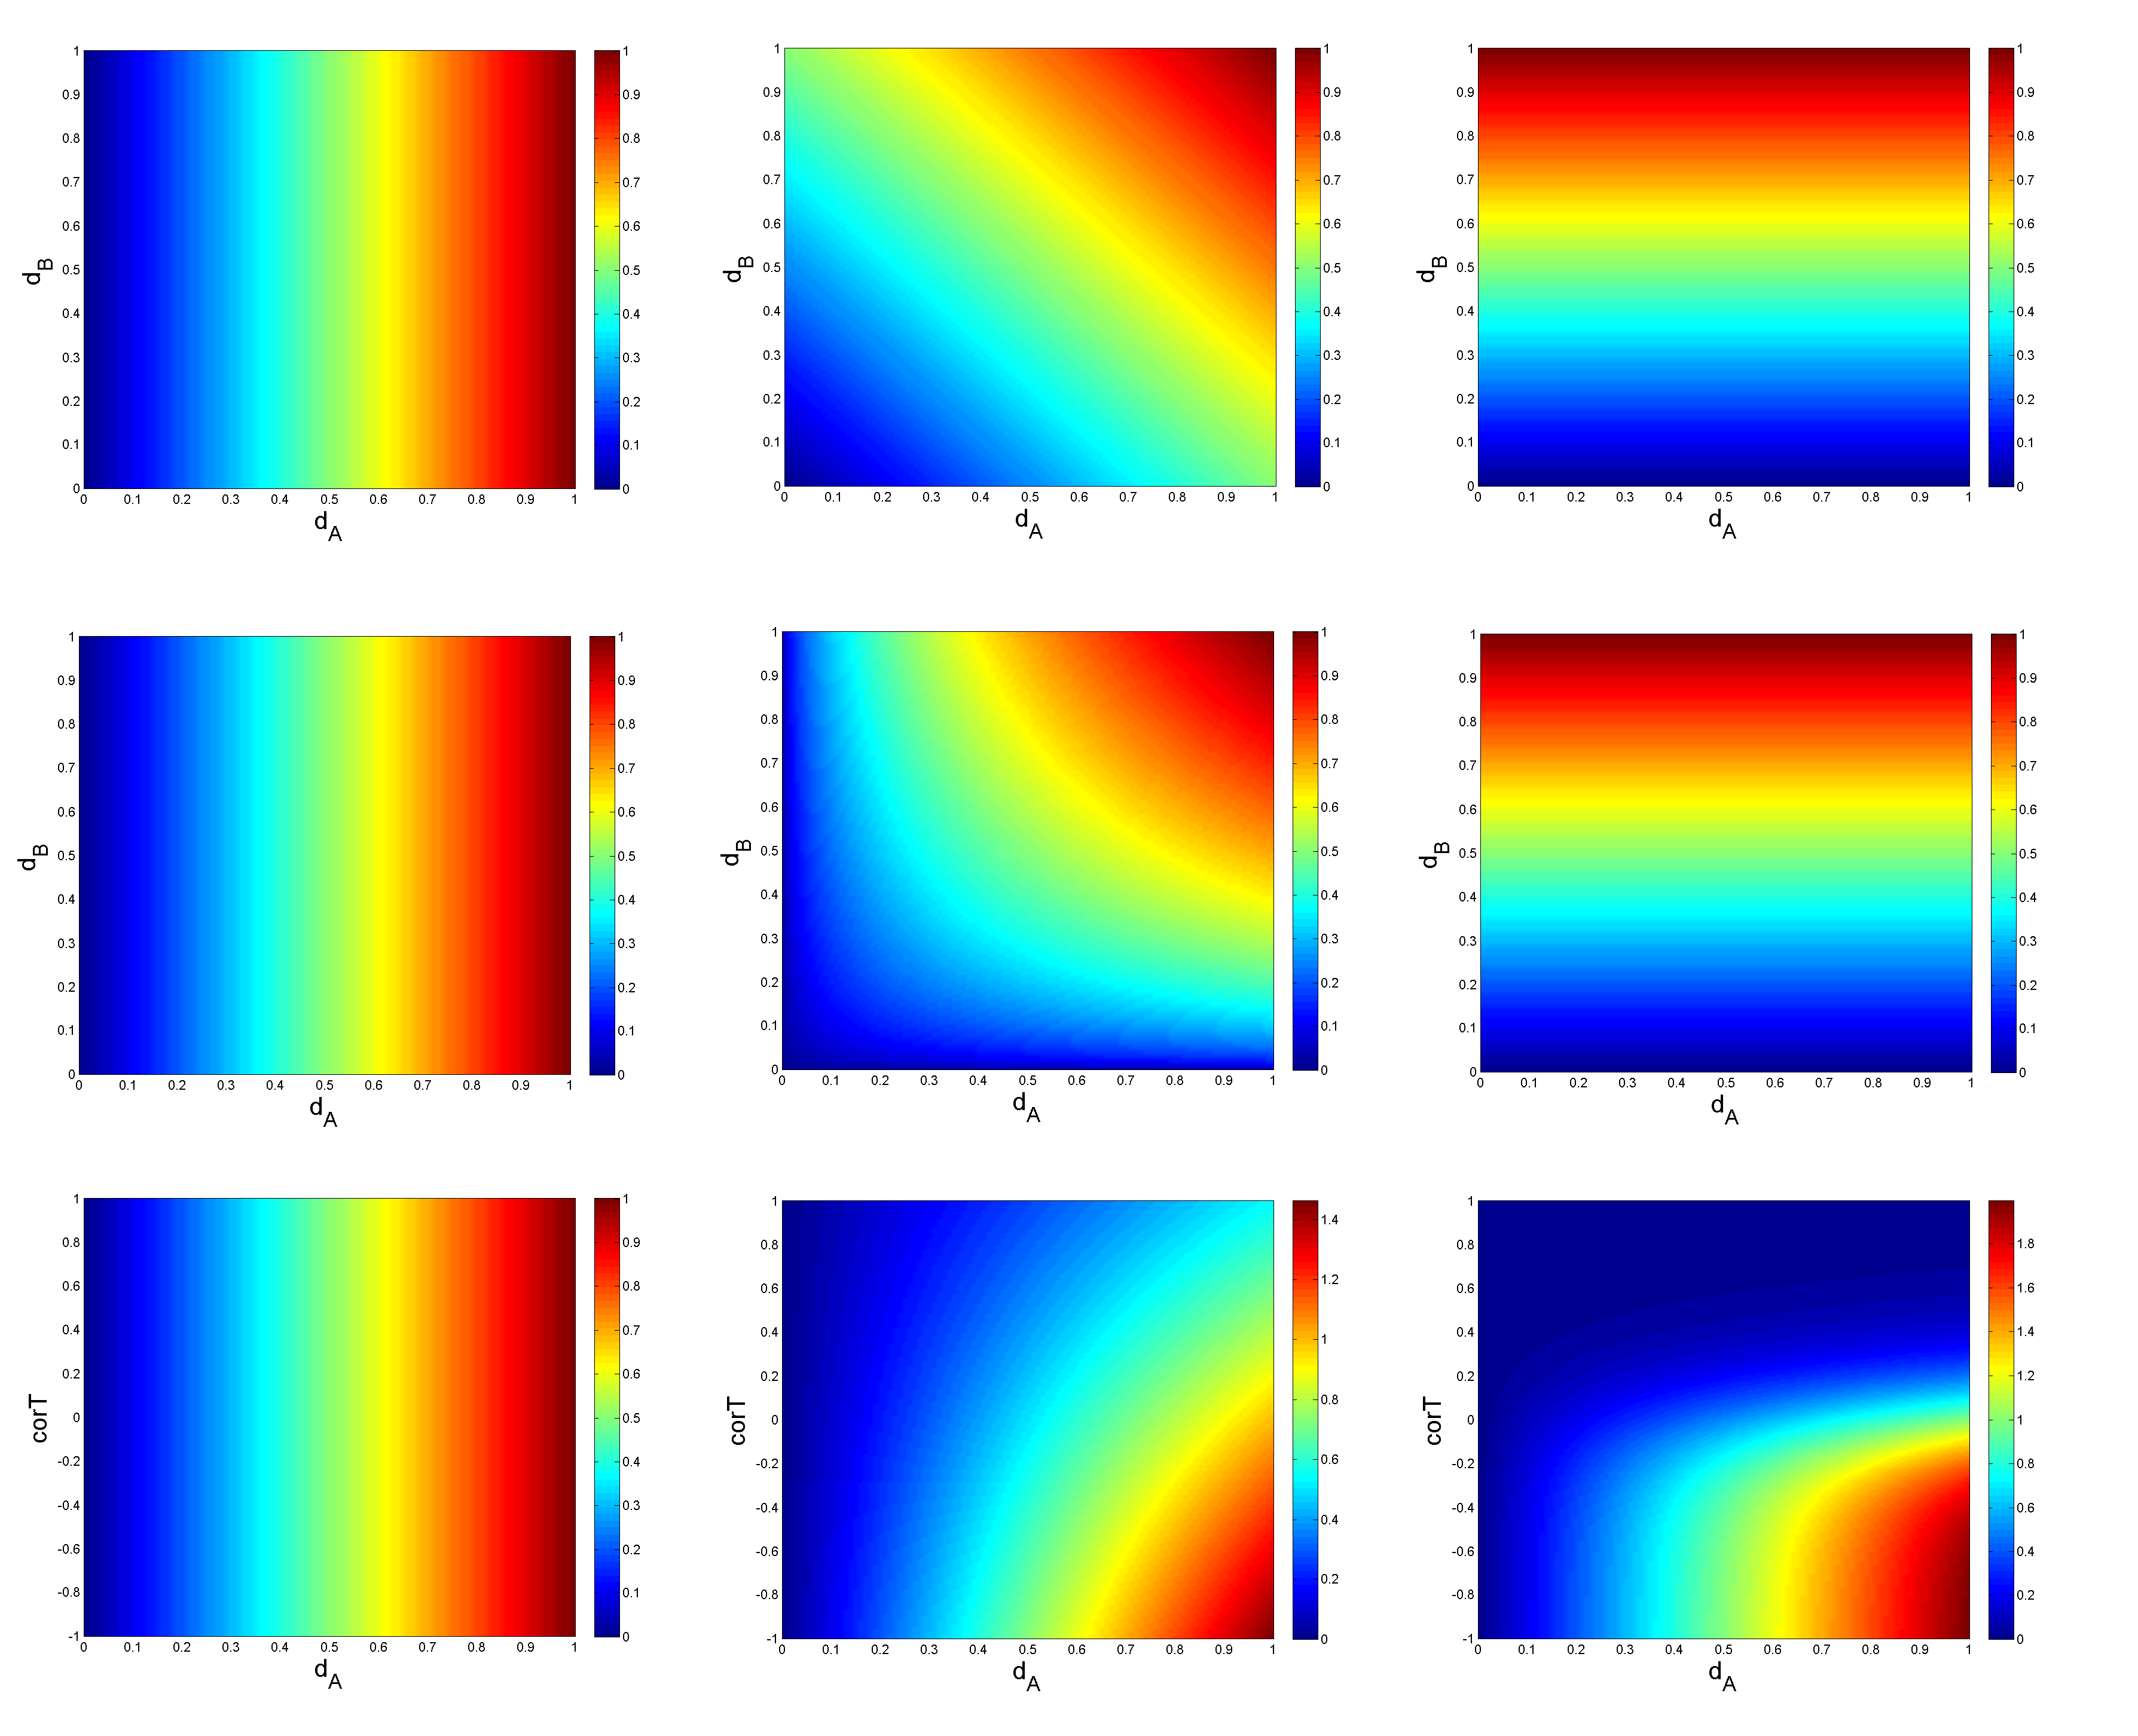
\includegraphics[width=1\linewidth]{images/CombinedMetrics}
	\caption{Contour plot of the resulting combined metrics: $D_{Lin}$ ($1^{st}$ line), $D_{Geom}$ ($2^{nd}$ line) and $D_{Sig}$ ($3^{rd}$ line), for different value of $\alpha$ ($D_{Sig}$: $\alpha=0;1;6$ and $D_{Lin}$ and $D_{Geom}$: $\alpha=0;0.5;1$). For $D_{Sig}$, the first and second dimensions are respectively the amplitude-based metrics $d_A$ and the temporal correlation $corT$; for $D_{Lin}$ and $D_{Geom}$, they correspond to $d_A$ and the behavior-based metric $d_B$.}
	\label{fig:ContourLine}
\end{figure}
\mycomment[MR]{Ajouter sur la figure la valeur de $\alpha$ et le nom des métriques pour une meilleure visibilité}

%-----------------------------------------------------------------------------
\section{Metric Learning}
%\begin{itemize}
%	\item Placer le contexte : travaux réalisés dans le cadre de la classification de données statiques.
%	\item Présenter l'intuition du Metric Learning sur la base des travaux de Weinberger.
%	\item Donner la terminologie (target, imposter, push, pull)
%	\item Objectif : push des imposters et pull des targets
%	\item Formalisation du problème (optimisation)
%	\item Limites:
%	\begin{itemize}
%		\item On apprend les poids d'une distance de Mahalanobis
%		\item L'apprentissage ne prend pas en compte l'aspect multi-modal dans les données
%	\end{itemize}
%\end{itemize}

The problem in this PhD is to define a metric that can be learnt in order to optimize the performance of the $k$-NN classifier. In this section, we first make a state of the art of Metric Learning propositions. Then, we focus on the framework proposed by Weinberger \& Saul for Large Margin Nearest Neighbor (LMNN) classification \cite{Weinberger2009}.

\subsection{State of the art}
In the case of static data, many work have demonstrated that $k$-NN classification performances depends highly on the considered metric and can be improved by learning an appropriate metric \cite{Shental2002,Goldberger2004,Chopra2005}. Metric Learning can be defined as a process that aims to learn a distance from labeled examples by making closer samples that are expected to be similar, and far away those expected to be dissimilar.

\todo[inline]{A faire, le positionnement du Metric Learning avec l'aide du papier PRL} 
%Similar and dissimilar samples, are inherently task- and application dependent, generally given a priori and fixed during the learning process. From the surge of recent research in metric learning, one can identify mainly two categories: the linear and non linear approaches. The former is the most popular, it defines the majority of the propositions, and focuses mainly on the Mahalanobis distance learning. The latter relies on non linear Metric Learning, although more expressive, the optimization problems are more expensive to solve in general.
%
%Contrary to flat data, Metric Learning for structured data (e.g. sequence, time series, trees, graphs) remains less numerous. While for sequence data most of the works focus on string edit
%distance to learn the edit cost matrix [21, 20], Metric Learning for time series is still in its infancy. Without being exhaustive, major recent proposals rely on weighted variants of dynamic time warping to learn alignments under phase or amplitude constraints [22, 23, 24], or enlarging temporal alignments to learn discriminative matching guided by local variance/covariance [25].


\subsection{Large Margin Nearest Neighbors (LMNN)}
Let $\textbf{X}=\{\textbf{x}_i,y_i\}_{i=1}^N$ be a set of $N$ static vector samples, ${\textbf{x}_i \in \mathbb{R}^{p}}$, $p$ being the number of descriptive features and $y_i$ the class labels. Weinberger \& Saul proposed in~\cite{Weinberger2009} an approach to learn a dissimilarity metric $D$ for a large margin $k$-NN in the case of static data. 

Large Margin Nearest Neighbor (LMNN) approach is based on two intuitions: first, each training sample $\textbf{x}_i$ should have the same label $y_i$ as its $k$ nearest neighbors; second, training samples with different labels should be widely separated. For this, the concept of \textbf{target} and \textbf{imposters} for each training sample $\textbf{x}_i$ is introduced. Target neighbors of $\textbf{x}_i$, noted $j \rightsquigarrow i$, are the $k$ closest $\textbf{x}_j$ of the same class $(y_j=y_i)$, while imposters of $\textbf{x}_i$, denoted, $l \nrightarrow i$, are the $\textbf{x}_l$ of different class $(y_l \neq y_i)$ that invade the perimeter defined by the farthest targets of $\textbf{x}_i$. 
Mathematically, for a sample $\textbf{x}_i$, an imposter $\textbf{x}_l$ is defined by an inequality related to the targets $\textbf{x}_j$: $\forall l, \exists j \in j \rightsquigarrow i /$
\begin{align}
D(\textbf{x}_i,\textbf{x}_l) &\leq D(\textbf{x}_i-\textbf{x}_j) + 1
\end{align}
% ||L(\textbf{x}_i-\textbf{x}_l)||^2 & \leq ||L(\textbf{x}_i-\textbf{x}_j)||^2 + 1 \\
Geometrically, an imposter is a sample that invades the target neighborhood plus one unit margin as illustrated in Fig. \ref{fig:TargetImposterRepresentation}. Note that the target neighborhood is defined with respect to an initial metric. Without prior knowledge, L2 norm is often used. Metric Learning by LMNN aims to minimize the number of impostors invading the target neighborhood. By adding a margin of safety of one, the model is ensured to be robust to small amounts of noise in the training sample (large margin). The learned metric $D$ pulls the targets and pushes the imposters as shown in Fig. \ref{fig:TargetImposterRepresentation}.

\begin{figure}[h!]
	\begin{minipage}[b]{1.0\linewidth}
		\centering
		\centerline{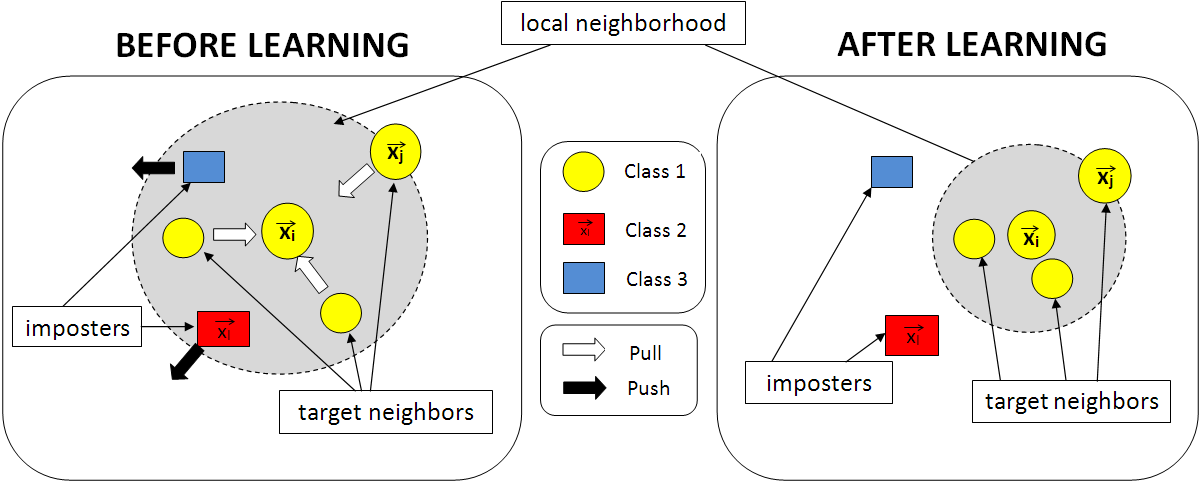
\includegraphics[width=0.8\linewidth]{./images/TargetImposterRepresentationCao}}
	\end{minipage}
	\caption{Pushed and pulled samples in the $k=3$ target neighborhood of $\textbf{x}_i$ before (left) and after (right) learning. The pushed (vs. pulled) samples are indicated by a white (vs. black) arrows (Weinberger \& Sault~\cite{Weinberger2009}).}
	\label{fig:TargetImposterRepresentation}
\end{figure}

LMNN approach learns a Mahalanobis distance $D$ for a robust $k$-NN. We recall that the $k$-NN decision rule will correctly classify a sample if its $k$ nearest neighbors share the same label (Section \ref{sec:kNN}). 
The objective of LMNN is to increase the number of samples with this property by learning a linear transformation $\textbf{L}$ of the input space ($\textbf{x}_i=\textbf{L}.\textbf{x}_i$) before applying the $k$-NN classification:
\begin{equation}
	D(\textbf{x}_i,\textbf{x}_j) = ||\textbf{L}(\textbf{x}_i,\textbf{x}_j)||_2^2
	\label{eq:lin}
\end{equation}
\noindent Commonly, the squared distances can be expressed in terms of the square matrix:
\begin{equation}
\textbf{M} = \textbf{L}'\textbf{L}
\end{equation}
It is proved that any matrix \textbf{M} formed as below from a real-valued matrix \textbf{L} is positive semidefinite (i.e., no negative eigenvalues) \cite{Weinberger2009}. Using the matrix \textbf{M}, squared distances can be expressed as:
\begin{equation}
D(\textbf{x}_i,\textbf{x}_j) = (\textbf{x}_i-\textbf{x}_j)\textbf{M}(\textbf{x}_i-\textbf{x}_j)
\end{equation}
Learning the linear transformation $\textbf{L}$ is thus equivalent to learn the corresponding Mahalanobis metric $D$ parametrized by $\textbf{M}$. This equivalence leads to two different approaches to metric learning: we can either estimate the linear transformation $\textbf{L}$, or estimate a positive semidefinite matrix $\textbf{M}$. LMNN solution refers on the latter one.



%\subsection{Intuition}
%%\begin{itemize}
%%	\item Se placer dans le contexte kNN
%%\end{itemize}
%
%Intuitively, the algorithm is based on the simple observation that the kNN decision rule will correctly classify an example if its k-nearest neighbors share the same label. The algorithm attempts to increase the number of training examples with this property by learning a linear transformation of the input space that precedes kNNclassification using Euclidean distances. The linear transformation is derived by minimizing a loss function that consists of two terms. The first term penalizes large distances between examples in the same class that are desired as k-nearest neighbors, while the second term penalizes small distances between exampleswith non-matching labels. Minimizing these terms yields a linear transformation of the input space that increases the number of training examples whose k-nearest neighbors have matching labels. The Euclidean distances in the transformed space can equivalently be viewed as Mahalanobis distances in the original space. We exploit this equivalence to cast the problem of distance metric learning as a problem in convex optimization. Our
Mathematically, it can be formalized as an optimization problem involving two competiting terms for each sample $\textbf{x}_i$: one term penalizes large distances between nearby inputs with the same label (pull), while the other term penalizes small distances between inputs with different labels (push). For every $\textbf{x}_i$, this implies a minimization problem:
\begin{equation}
\begin{aligned}
&\displaystyle 		\min_{w,\xi}\underbrace{
	\sum\limits_{i,j \rightsquigarrow i}
	D(\textbf{x}_{i},\textbf{x}_{j})
}_{pull}
+
\underbrace{
	C\sum\limits_{i,j \rightsquigarrow i,l} \frac{1+y_{il}}{2}.\xi_{ijl}
}
_{push} \\
&\text{s.t.  } \forall j \rightsquigarrow i, y_l\neq y_i, \\
& D(\textbf{x}_{i},\textbf{x}_{l})-D(\textbf{x}_{i},\textbf{x}_{j}) \geq 1-\xi_{ijl} \\
& \xi_{ijl} \geq 0 \\
\label{eq:OptimizationProblem}
\end{aligned}
\end{equation}
\noindent where $C$ is a trade-off between the push and pull term and $y_{il}=-1$ if $y_i=y_l$ (same class) and $+1$ otherwise (different classes). Generally, the parameter $C$ is tuned via cross validation and grid search. Similarly to Support Vector Machine (SVM) approach, slack variables $\xi_{ijl}$ are introduced to balance the effect of noise in real data. 

Many parallels can be made between LMNN and SVM: both are convex optimization problem based on a regularized and a loss term. Thus, some authors extends the approach to work in non-linear feature spaces by using the “kernel trick” \todo{ref}. LMNN differs from SVM in which $k$-NN classification replaces linear classification and LMNN requires no modification for multiclass problems.





%-----------------------------------------------------------------------------
\section{Conclusion of the chapter}
To cope with modalities inherent to time series, we review in this chapter several unimodal metrics dedicated to time series. Depending on the considered modality (amplitude, behavior, frequency), adapted metrics for time series have been proposed in the literature such as the Euclidean distance $d_A$, the Temporal correlation $d_B$ or the Fourier-based distance $d_F$.

In practice, real time series may be subjected to delays. They need to be re-aligned before any analysis task. For that, the Dynamic Time Warping (\textsc{dtw}) algorithm has been used usually. To capture local characteristics, the previous metrics $(d_A, d_B, d_F)$ can be computed on smaller intervals. Many strategies exist such as the dichotomy or the sliding window.

However, all of these metrics only include one modality and at a particular scale. In general, several modalities may be implied in real data. Some authors proposed to combine temporal metrics together. They mainly combine the Euclidean distance $d_A$ and the Temporal correlation $d_B$. As $k$-NN performances is impacted by the choice of the metric, other work propose in the case of static data to learn the metric in order to optimize the $k$-NN classification. In the following, we extend this framework to learn a combined metric for large margin $k$-NN classification of time series.

% After that, we will take an insight on Metric Learning approaches which aims to learn a metric that makes closer samples that are expected to be similar, and far away those expected to be dissimilar.


% In the next section, we present a new temporal metric learning framework for a robust nearest neighbors time series classification and give, in Section 4, a solution to learn a holistic temporal metric that combines efficiently several temporal modalities at different scales.


% Local optimal metrics and nonlinear modeling of chaotic time series
% Integration of local and global shape information


%%% Local Variables: 
%%% mode: latex
%%% TeX-master: "../roque-phdthesis"
%%% End: 
